\subsection{Linear Regression}

El \cite{Sklearn Linear Regression} es un modelo lineal que permite ajustar a un conjunto de datos y utilizarlo para hacer predicciones. Este modelo se basa en la minimización de la suma de los cuadrados de los residuos entre las predicciones del modelo y los datos observados, y se puede utilizar tanto para resolver problemas de regresión como de clasificación binaria. En este modelo no se pueden modificar los parametros, por lo que la experimentación es bastante sencilla. Se ha entrenado el modelo con los datos estandarizados y con la resta de las variables objetivo, hecho que nos ha permitido obtener los siguientes resultados.

\begin{figure}[H]
    \centering
    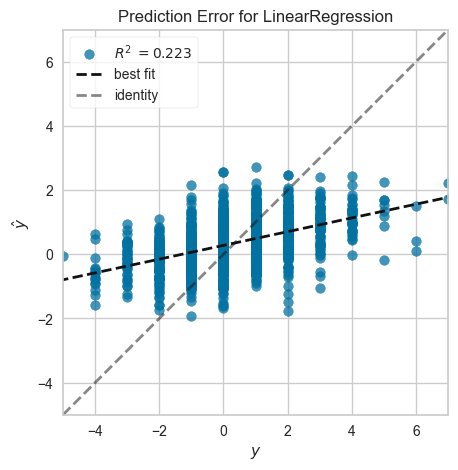
\includegraphics[width=\smallSize]{images/linearModelLinearRegression.png}
    \caption{Linear Regression: Prediccion}
    \label{Modelos-Lineales-Linear-Regression-Prediccion-Error}
\end{figure}

En la Figura \ref{Modelos-Lineales-Linear-Regression-Prediccion-Error} podemos ver como los resultados obtenidos no son demasiado satisfactorios. Esta conclusion se puede obtener tanto graficamente como analiticamente, consultando el valor $R^2$ que equivale a $0.223$. 
\newline

Además, se realizará con todos los modelos es el calculo del tiempo medio de entrenamiento, en este caso, el modelo de regresión lineal tiene un tiempo de entrenamiento medio de $0.013$ segundos. Por otra parte, al ejecutar la Validación cruzada al modelo entrenado se han obtenido, de media, un valor de $0.216$. Si nos fijamos en los valores obtenidos por cada uno de los pliegues que se ha realizado al conjunto de datos encontramos en el Cuadro \ref{Modelos-Lineales-Linear-Regression-Validacion-Cruzada}.

\begin{table}[h]
    \centering
    \begin{tabular}{lccccc}
        \textbf{Pliegue} & 1 & 2 & 3 & 4 & 5 \\
        \textbf{Resultado} & 0.25609482 & 0.1231758 & 0.25783003 & 0.16857474 & 0.27594974
    \end{tabular}
    \caption{Linear Regression: Resultados Validación Cruzada}
    \label{Modelos-Lineales-Linear-Regression-Validacion-Cruzada}
\end{table}